%
% Copyright (C) 2011 Agostino De Marco
%                    <agostino dot demarco at unina dot it>
%                    Roberto Giacomelli
%                    <giaconet dot mailbox at gmail dot com>
%
%    This work may be distributed and/or modified under the
%    conditions of the LaTeX Project Public License, either
%    version 1.3 of this license or any later version.
%    The latest version of this license is in
%    http://www.latex-project.org/lppl.txt and version 1.3
%    or later is part of all distributions of LaTeX version
%    2005/12/01 or later.
%
% This work has the LPPL maintenance status `maintained'.
% 
% The Current Maintainer of this work are Agostino De Marco
% and Roberto Giacomelli
%
\documentclass{standalone}
\usepackage{pgfplots}
\usepgfplotslibrary{polar}

\begin{document}
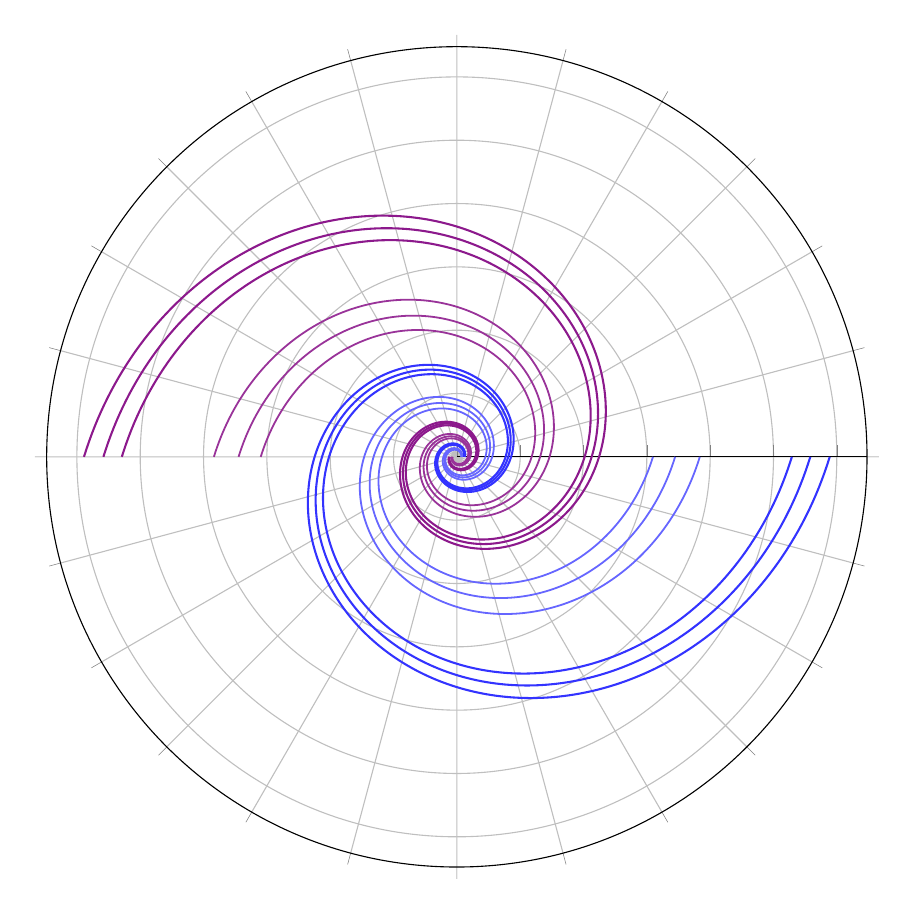
\begin{tikzpicture}
\begin{polaraxis}[
  xticklabels=\empty,
  ytick={0,40,...,400},
  yticklabels=\empty,
  width=12cm,
  samples=600,
  mark=none,
  domain=0:720]
       
\foreach \phase in {180,200,220}
   \addplot[line width=.65pt,blue!60]
       {exp((x+\phase)*0.0053548)};

\foreach \phase in {280,290,300}
   \addplot[line width=.75pt,blue!80]
       {exp((x+\phase)*0.0053548)};
       
\foreach \phase in {180,200,220}
   \addplot[line width=.65pt,violet!80]
       {-exp((x+\phase)*0.0053548)};

\foreach \phase in {280,290,300}
   \addplot[line width=.75pt,violet!90]
       {-exp((x+\phase)*0.0053548)};
\end{polaraxis}
\end{tikzpicture}
\end{document}